\documentclass{beamer}
\usetheme{UWr_blue}

\usepackage [utf8]{inputenc}
\usepackage {polski}
\usepackage {color,graphicx}
\usepackage {amssymb}
\usepackage {enumerate}
\usepackage {amsmath}
\usepackage {caption}
\usepackage {subcaption}
\usepackage {geometry}
\usepackage {empheq}
\usepackage {wrapfig}
\usepackage {float}

\title{Przykładowa prezentacja tematu WFA}
\author{Krzysztof Cach}
\institute{Instytut fizyki teoretycznej}
\date{Wrocław, \today}

\setbeamercovered {invisible}

\begin{document}

\begin{frame}
	\titlepage{}
\end{frame}

\begin{frame}
\frametitle{Przykładowe elementy:}
\tableofcontents
\end{frame}

\section{Enumerate}
\begin{frame}
	\frametitle{Enumerate}
	\begin{enumerate}
	\item item1
	\item item2
	\item item3
	\end{enumerate}
\end{frame}

\section{Itemize}
\begin{frame}
	\frametitle{Itemize}
	\begin{itemize}
	\item item1
	\item item2
	\item item3
	\end{itemize}
\end{frame}

\section{Blocks}
\subsection{alert}
\subsection{standard}
\subsection{example}

\begin{frame}
	\frametitle{Blocks}
	\begin{alertblock}{Alert block}
		Body
	\end{alertblock}

	\begin{block}{Standard block}
		Body
	\end{block}

	\begin{exampleblock}{Example block}
		Body
	\end{exampleblock}
\end{frame}

\section{Equation}
\begin{frame}
	\frametitle{Equation}
	\begin{equation}
	\theta_i(t + \delta t) = \left< \theta (t) \right> _{S(i)} + \xi
	\end{equation}
	
	\begin{equation}
	\Phi = \frac{1}{N} \left| \sum_j \vec{v}_j \right|
	\end{equation}
\end{frame}

\section{Graphics}
\begin{frame}
	\frametitle{Graphics}
	\begin{figure}[H]
	\caption{Czirók, Vicsek - Physica A 281 (2000) 17-29}
	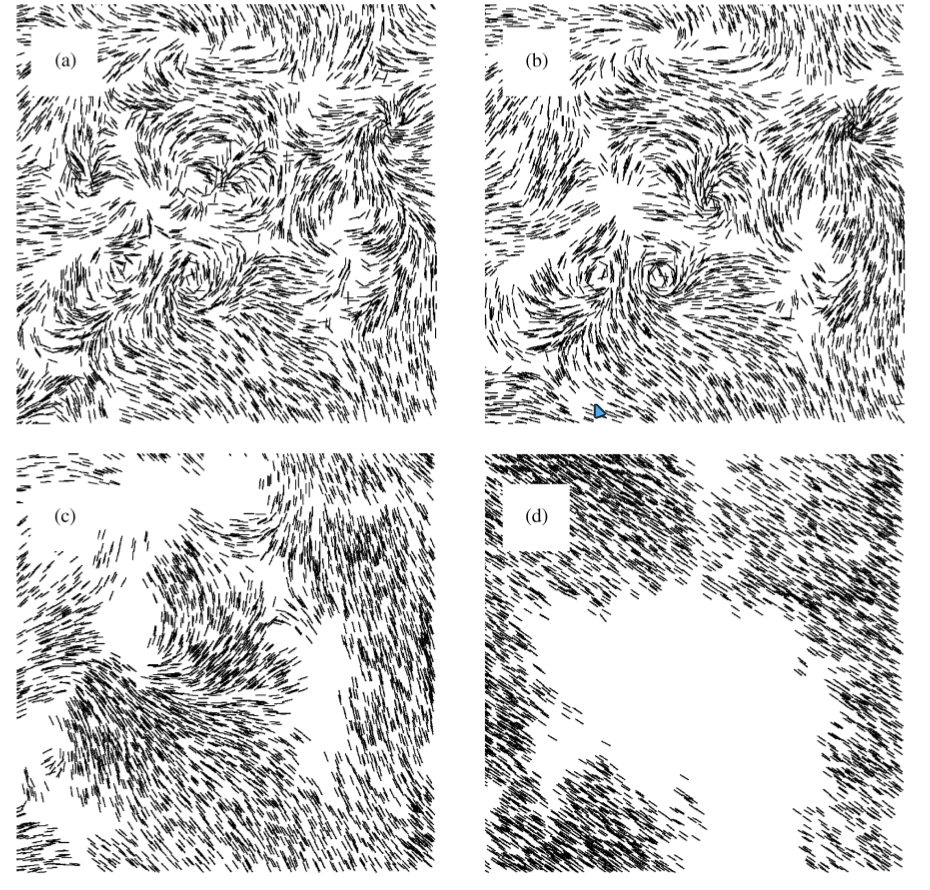
\includegraphics[width=0.7\textwidth, height=0.7\textheight]{images/wyniki.png}
	\end{figure}	
\end{frame}
\end{document}
